\documentclass[nochap, headernames]{config/ejercicios}

\title{Prácticas Filogenia molecular (PHYLO)}
\author{Sandra Mingo Ramírez}
\date{2024/25}

\usepackage[all]{nowidow}
\usepackage{listing}
\usepackage{color}
\usepackage{tabularx}
\usepackage{multirow}
\usepackage{makecell}
\usepackage{amsmath}
\usepackage{array}
\usepackage{hyperref}

\begin{document}

\maketitle

%Programas adicionales: Genius, Ugene (alternativa gratuita de genius), Phylemon
%SeaView es un programa muy simple que permite arrastrar cualquier archivo para abrir alineamientos o árboles. Permite realizar funciones simples, pero que podrían ser laboriosas en otros programas, como por ejemplo eliminar el nucleótido en la posición X. 

\section{Formatos de archivos  filogenéticos y alineamientos}
El objetivo es familiarizarse con la conversión de formatos de archivo, diferentes métodos de alineación, eliminación de posiciones ambiguamente alineadas, edición de matrices y traducción de secuencias de ADN a proteínas.
\begin{enumerate}
\item Alinea el conjunto de datos utilizando MAFFT (en línea) con la estrategia Auto. Guarda el alineamiento resultante en formato fasta. \footnote{Los archivos fasta empiezan con el símbolo > seguido de un descriptor de la secuencia. Después, empieza la secuencia en una nueva línea. Cuando termine, hay un nuevo prompt con un nuevo descriptor.}
\item Alinea el conjunto de datos utilizando CDS-ProtAl: Utilidades > Utilidades de Alineación > CDS-ProtAl > Examinar servidor > Cargar nuevo archivo, Seleccionar formato > Secuencias no alineadas > Cargar > Aceptar, Parámetros > Mantener huecos, Código genético > Estándar. Ejecutar.
\item Compara las dos alineaciones resultantes utilizando SeaView. Arrastra el archivo de salida MAFFT. Luego Archivo > Nueva Ventana, arrastre el archivo de salida CDS-ProtAl.
\item Utiliza TrimAl para eliminar las posiciones ambiguamente alineadas. Esto puede hacerse automáticamente (redirigiendo el archivo resultante de CDS-ProtAl en Phylemon) o manualmente (Utilidades > Utilidades de Alineación > TrimAl). Selecciona Método 'sin huecos' para este ejercicio.
\item Utiliza SeaView para traducir una matriz de secuencia de nucleótidos a aminoácidos. Utiliza el conjunto de datos de TrimAl. Arrastra el archivo. Props > Ver como proteínas. Archivo > Guardar prot alineación. \textbf{Nota}: Si es necesario, se puede cambiar el código genético: Edit > Set genetic code.
\item Familiarízate con la conversión de formatos de archivo utilizando ALTER. Introduce el archivo de entrada en formato fasta (paneles de la izquierda): 
\begin{enumerate}
\item Seleccionar formato > Autodetectar
\item Cargar o pegar MSA > Seleccionar sistema operativo > Linux / Mac OS X. Seleccione el de salida (paneles derechos): Seleccionar programa > RAxML, formato > PHYLIP, Convertir
\item Guardar MSA convertido > Seleccionar sistema operativo > Linux / Mac OS X, Guardar
\item Repita la exportación al formato Nexus (Seleccione programa > MrBayes, formato > NEXUS).
\end{enumerate}
\end{enumerate}

MAFFT es un programa muy utilizado. Tiene una versión descargable y una versión en línea que permite utilizar los servidores localizados en Japón. La versión en línea cuenta con un cuadro donde pegar los datos, aunque también se puede seleccionar un archivo desde el disco duro. En nuestro caso, subiremos el archivo \texttt{HRSV-A\_modif\_RAW.fas}. Se pueden elegir algunas opciones de estética, como el uso de mayúsculas y minúsculas (la convención es poner los nucleótidos en minúscula y los aminoácidos en mayúscula), la dirección de las secuencias (se le puede pedir al programa que compruebe y ajuste la direccionalidad, aunque consume más recursos y tarda más tiempo) y el orden de la salida. Poner un nombre al trabajo puede ser útil cuando se van a lanzar varios trabajos simultáneamente. También permite poner una dirección de correo que notifique cuando se ha terminado de analizar un trabajo que vaya a tardar mucho para evitar tener que estar con la pestaña del ordenador abierta. Entre la configuración avanzada, se puede seleccionar la estrategia. Los métodos progresivos van alineando las secuencias en parejas y las van alineando poco a poco, añadiendo gaps donde toque según ese alinamiento. Los métodos iterativos, después de alinear todas las secuencias, vuelve al principio a reevaluar el alineamiento y mejorándolo. Por este motivo, los métodos iterativos son más lentos y se recomiendan para sets de pocas secuencias. También hay una estrategia automática que evalúa cuatro de los algoritmos según el tamaño de los datos y utiliza uno u otro. El resultado del alineamiento después de darle al botón de Submit es el que aparece en la imagen \ref{fig:mafft-result}.

\begin{figure}
\centering
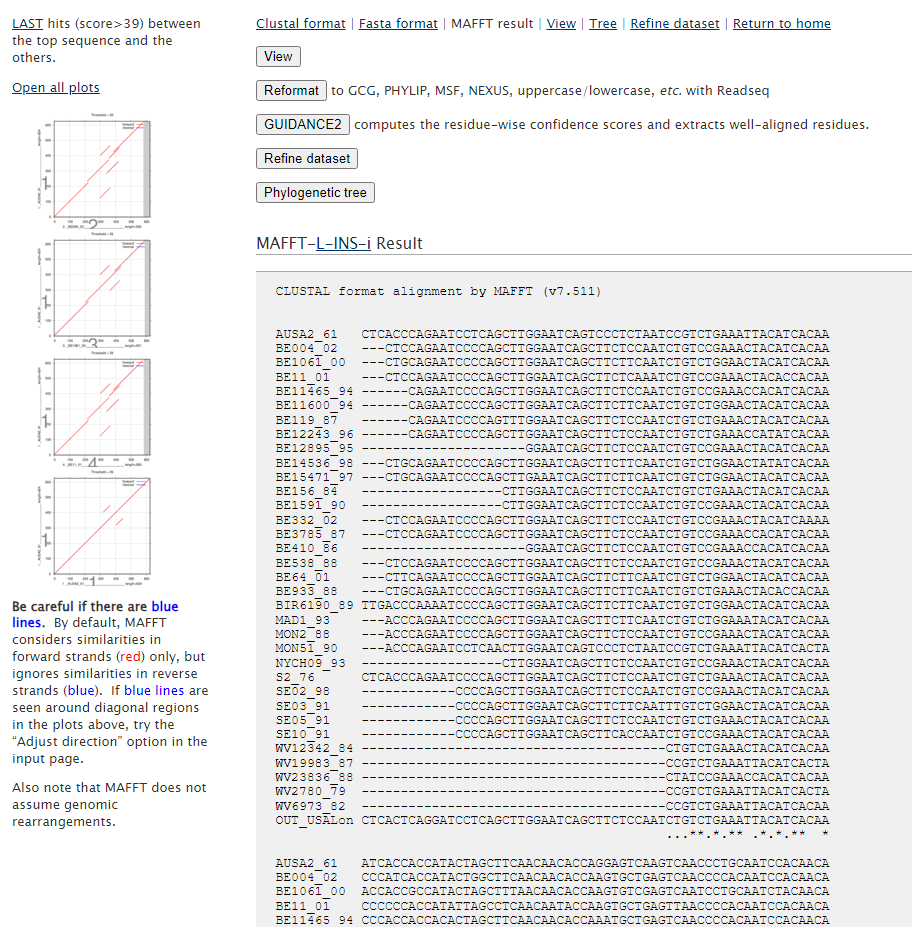
\includegraphics[width = \linewidth]{figs/mafft-result.png}
\caption{Resultado del alineamiento del fichero HRSV-A. La parte de la izquierda muestra unos gráficos de similitud. Debería estar todo en rojo, ya que si hay alguna línea en azul, eso indicaría que hay secuencias invertidas y que habría que reevaluar el alineamiento ajustando la direccionalidad.}
\label{fig:mafft-result}
\end{figure}

Para guardar el alineamiento, lo más cómodo es pulsar el botón de \texttt{Fasta format} en la parte superior. Este alineamiento lo podemos visualizar entonces en el programa de SeaView o en \href{http://phylemon.bioinfo.cipf.es/}{Phylemon}. \footnote{Tradicionalmente funcionaba bien en Google Chrome y daba error o no cargaba en otros navegadores. Ahora parece ser que es al revés; no carga usando Google Chrome, pero en Firefox funciona bien.} Este último tiene en el cluster programas de terceros para realizar alineamientos, árboles filogenéticos, test evolutivos y pipelines para combinarlos, pero también otras utilidades exclusivas. Dentro de las utilidades de alineamientos, hay tres programas: ConcatenAl permite concatenar los alineamientos, CDS-ProtAl sirve para traducir proteínas desde las secuencias codificantes, y TrimAl permite eliminar partes de la secuencia que están alineadas de forma dudosa o que tienen gaps. Nosotros vamos a utilizar CDS-ProtAl, donde podemos pegar una secuencia o subirla. Al subir un archivo, hay que seleccionarlo y decir el tipo de archivo que es (secuencia alineada, sin alinar, árbol, etc). Los parámetros que se pueden seleccionar son mantener o no los gaps y traducir la secuencia sin alinearla. También pide el código genético para poder traducir las proteínas. En nuestro caso del virus respiratorio sincitial humano, utilizaremos el código genético estándar. Una vez terminado el trabajo, nos podemos descargar los ficheros resultantes pulsando sobre el nombre o haciendo click derecho y "guardar enlace como". Aunque el formato sea out\_ali, se puede cambiar manualmente a fasta y visualizar con SeaView. 

Hay algunos casos en los que las regiones no alineadas pueden producir mucho ruido filogenético. Para eso, existen programas que permiten seleccionar bloques de secuencia conservada, como Gblocks o TrimAl. Desde Phylemon, se puede redirigir el resultado obtenido con CDS-ProtAl directamente a TrimAl (y otras herramientas) mediante un desplegable, facilitando así el trabajo y evitando tener que descargar los archivos intermedios y temporales. Antes de lanzar el trabajo con TrimAl, permite seleccionar la eliminación de secuencias de baja similitud o calidad antes de quitar las posiciones. Hay varios métodos para quitar los gaps: "no gaps" quita todas las posiciones que tengan un gap,"no all gaps" quita las posiciones que sólo sean gaps y no tengan ninguna secuencia, y "gappyout" quita las posiciones que tienen más gaps de lo esperado. 

Desde SeaView se puede también traducir una secuencia a proteínas mediante Props y el check de "ver como proteínas". En "File" se puede guardar el archivo. En algunos casos, algunas posiciones son muy variables (por ejemplo, las terceras posiciones de los genes mitocondriales, que tienen tantos cambios superimpuestos que no aportan información filogenética), por lo que es mejor eliminar las posiciones antes de realizar los análisis. En SeaView, esto se puede hacer en Sites y Create Set. A continuación se puede seleccionar aquellas posiciones que se quieren. Por ejemplo, para eliminar las terceras posiciones, habría que utilizar la opción que selecciona la primera y segunda posición. Para guardar esta selección, en File hay una opción de Save selection.

\end{document}
